% !TEX root = ../thesis.tex
\section{Dosažené výsledky a jejich analýza}
\label{chap:construction:results}

Z provedené anylýzy plyne, že získaný EL korpus je odlišný od \uv{standardního} řečového korpusu, který se běžně používá k trénování obecných akustických modelů. Tyto modely jsou nezávyslé na řečníkovi a vyznačují se robustnostní. Je tedy otázka zda takovýto model nebude schopen pracovat s EL daty.

K ověření byl vytvořen TDNN akustický model (více o těchto modelech v části \ref{chap:asr:acoustic:DNN}), který byl natrénován daty z korpusu čítající $1000$ hodin promluv od velkého počtu řečníků. Celkový počet HMM stavů je \textbf{XXXX}.

Jazykový model je postaven na trigramech a k jeho natrénování posloužil textový korpus čítající velké množství novinových článků, webových reportáží, fílmových titulků a dalších textových záznamů. Slovník jazykového modelu čítá více než $1$ milion unikátních slov.

Testovacím vstupem vytvořeného ASR systému jsou data z EL korpusu. Celkový slovní přesnost, počítaná podle vzorce (\ref{eq:asr:decoding:acc}), dosáhla hodnoty $18,49\ \%$\footnote{Dosaženo na state-of-the-art ASR systému v době psaní práce. V době vytvoření EL korpusu (kolem roku 2011) převládaly HMM-GMM akustické modely. Tento systém dosáhl přesnosti na slovek $12,59\ \%$.}.

Dosažený výsledek zřetelně ilustruje odlišnost EL domény, protože obecný na řečníkovi nezávyslý systém s velkým jazykovým modelem není schopen obstojně rozpoznat EL promluvu.

Pokud jsou k natrénování akustického modelu (taktéž využívajícího TDNN síť) použita pouze data\footnote{Korpus byl náhodně rozdělen na trénovací a testovací sadu v poměru $90\ \%$ trénovací a $10\ \%$ testovací sada. Toto rozděleni je použito ve všech experimentech.} z EL korpusu, tak výsledná slovní přesnost dosáhla hodnoty $83,33\ \%$, opět počítáno podle vzorce (\ref{eq:asr:decoding:acc}). Jazykový model je identický jako v případě obecného systému. Dosažený výsledek demostruje výhodu vytvoření individuálního modelu v případě, že nejsou k dispozici data od velkého množství řečníků. Zároveň ukazuje schopnost akustického modelu namodelovat specifika EL řeči. Přestože je výsledek individuálního modelu výrazně lepší, než obecného modelu zpracovájící EL promluvy, tak zdaleka nedosahuje hodnot nejlepších ASR systémů, které jsou v ideálních podmínkách dosahovat více než $90\ \%$ slovní přesnosti.


%Z dosaženého výsledku je patrné, že EL doména je diametrálně odlišná od bežné řeči, pro které jsou ASR systémy vytvářeny. Navíc, pokud se vezme v potaz náročnost získání potřebných dat pro natrénování obecného modelu, tak se jako jediná schůdná varianta jeví vytváření individuálních modelů pro každého řečníka. To znamená, že model je trénovaný pouze z dat odpovídající konkreténímu řečníkovi a často i účelu použití. K vytvoření takového modelu je zapotřebí řádově méně dat, při dosažení podobného výkonu. Stinnou stránkou je případná menší robustnost modelu. Čistě logicky tento model bude fungovat pouze s konkrétním řečníkem a ještě jen v situacích, které odpovídají trénovacím datům. U řečníků s EL může navíc hrát velký vliv samotný EL. Již při nahrávání se ukázalo, že jeho pozice může nepříznivě ovlivnit kvalitu řeči. Tento problém by však neměl významně ovlivňovat kvalitu modelu, protože tento fenomém je obsažen v datech.

\subsection{Hledání optimálních parametrů baseline modelu}
\label{chap:construction:results:baseline}

%Co se však ukázalo jako potencionálně problematické, je stabilita parametrů produkované řeči v dlouhodobém časovém úseku. Více o tomto problému pak v části \ref{chap:construction:normalization:quality}. K zodpovězení nejdůležitější otázky, jestli takový model vůbec může fungovat, stačí získaná data z první etapy nahrávání a ta obsahují řeč s relativně konzistentními parametry.

V rámci ověřování funkčnosti infividuálního modelu je vhodné zkusit různé varianty k nalezení optimálních parametry modelu. Hlavními uvažovanými hyperparametry jsou vzorkovací frekvence audio nahrávek a počet \textit{HMM} stavů. Originální pořízené nahrávky mají vzorkovací frekvenci rovnu $44,1\ kHz$, pro úlohu rozpoznávání je to zbytečně moc, protože nejhodnotnější informace je obsažena ve frekvenčním pásmu do $4\ kHz$. Vyšší frekcence a priory ovlivňují zabarvení hlasu a další individuální charakteristiky. \cite{Psutka2006} Otázkou je vhodnější vzorkovací frekvence rovna $8\ kHz$ nebo lépe $16\ kHz$.

Počet stavů modelu ovliňuje množsví modelovaných trifónů, viz \ref{chap:asr:acoustic:HMM}. Čím více akustických jednotek je modelováno, tím více musí mít HMM model unikátních stavů. Stinnou stránkou je, že čím více stavů model má, tím více trénovacích dat je potřeba k natrénování robustního modelu. Celkem jsou uvažovány modely s $1024,\ 2048$ a $4096$ stavy.

%Jen pro vysvětlení je dobré zmínit, že \textit{HMM} stav představuje model jedné uvažované akustické jednotky (nebo skupiny jednotek s podobnými parametry). Počet stavů nám tedy říká, kolik takových jednotek model dokáže rozlišit. Čím více stavů, tím více jednotek (menších skupin) je modelováno. Teoreticky tak model s více stavy je lepší. Nicméně k natrénování jednotky je potřeba určité množství dat a tím pádem je pro model s vyšším počtem stavů logicky potřeba větší množství trénovacích dat. Samozřejmě fonetická sada neobsahuje $4096$ fonémů, neobsahuje ani $1024$ fonémů\footnote{Ve skutečnosti obsahuje 42 českých fonémů.}. U těchto modelů se pak používá nějaký druh \textit{n-gramové} reprezentace fonémů, nejčastěji pak trifóny.

Celkově je tak natrénováno $6$ modelů. K vytvoření akustických modelů je použit HTK-Toolkitu v3.4., který je určen k vytváření \textit{HMM} modelů za pomocí k-means, Viterbiho a Baum-Welsch algoritmu, více o trénování akustických modelů v části \ref{chap:asr:acoustic}. Při trénování je nejprve vytvořen monofónový akustický model s jedním gaussiánem pro každý stav. Ten poté slouží jako základ pro trifónové modely. Výsledný trifóvý model využívá směs gaussiánů, tak jak je to popsáno v \ref{chap:asr:acoustic:GMM}. Celý proces trénování znázorněn na obr. \ref{fig:construction:results:baseline:hmm:training}.

\begin{figure}[hbpt]
  \centering
  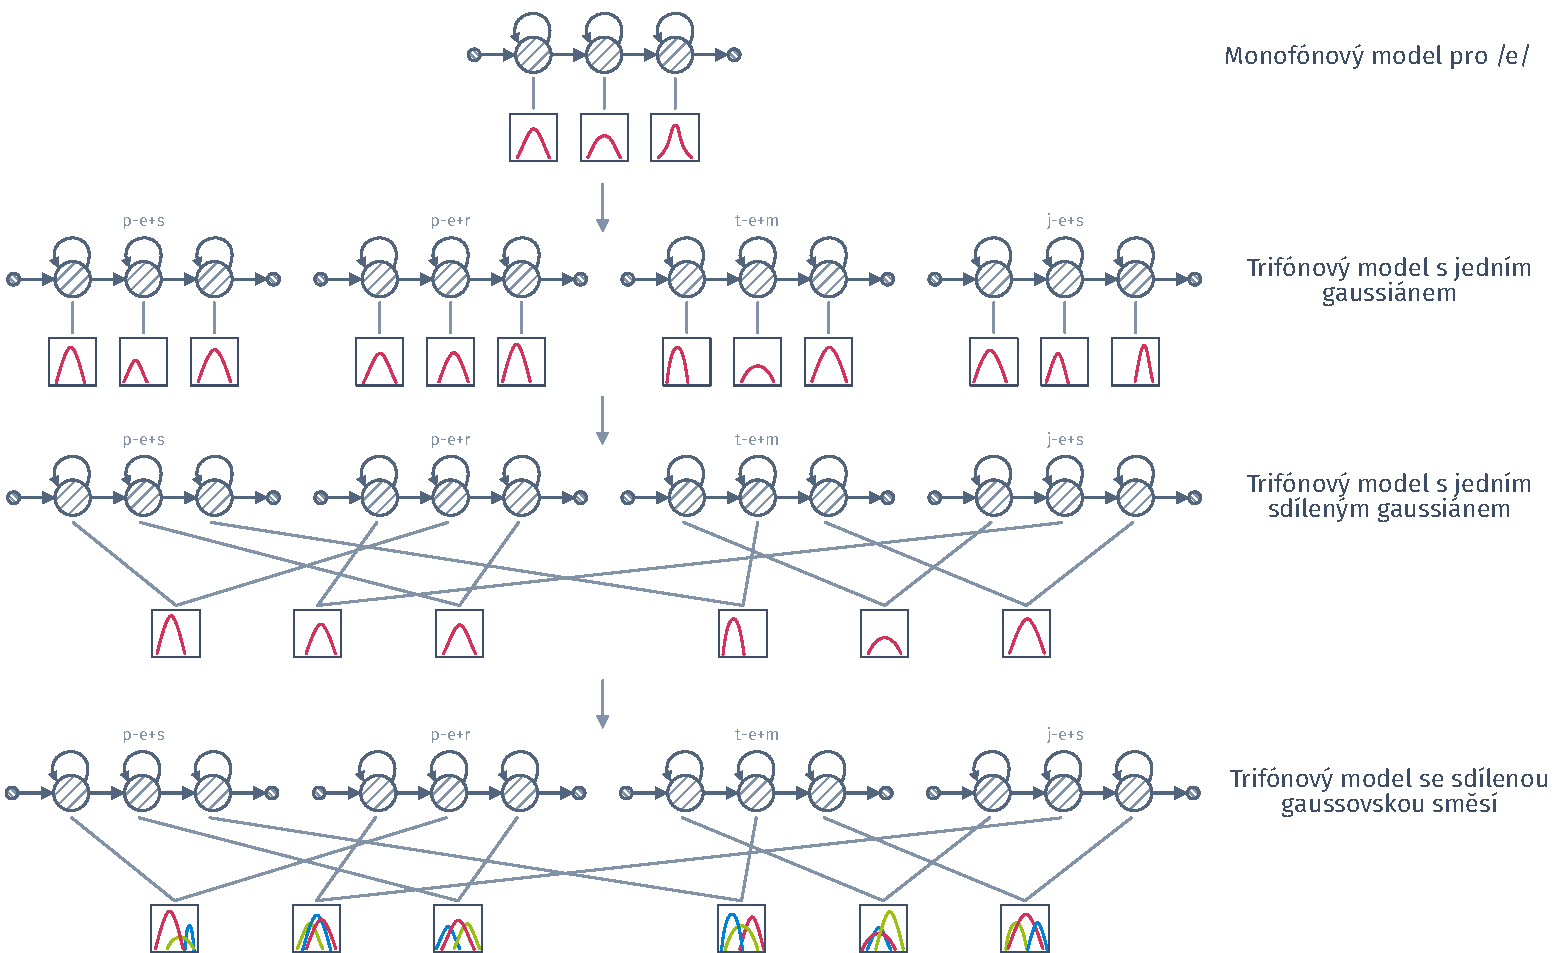
\includegraphics[width=0.9\textwidth]{./ch5-construction/img/hmm-training.pdf}
  \caption{Princip trénování HMM-GMM modelu}
  \label{fig:construction:results:baseline:hmm:training}
\end{figure}

Snahou je nalezení vhodných parametrů baseline modelu, zejména pak toho akustického. Z tohoto důvodu je jako jazykový model zvolen fonémový zerogramový jazykový model. Ten se vyznačuje stejnou pravděpodoností pro všechny možné výstupy modelu, fonémy. Tato pravděpodobnost je rovna $P(w_n) = 1/N$, kde $N=40$. Výstupem akustikého modelu jsou fonémy, pokud jazykový model má pro všechny možné výstupy stejnou pravděpodobnost, tak nijak neovlivní celkový výkon systému, viz \ref{chap:asr:decoding}. Výsledná přesnost je tedy a priory závislá na akustickém modelu. Akustická data byla parametrizována pomocí MFCC s 26 filtry, 12 kepstrálními koeficienty a energií. Příznakový vektor obsahuje první i druhou derivaci těchto koeficentů. Více o parametrizaci založené na procesu slyšení v části \ref{chap:asr:parametrization:hearing}.


% Funkce ASR systému lze popsat rovnící

% \begin{equation}
%   \argmax_W p\left(W | O\right) = \argmax_W p\left(O | W\right) p\left(W\right),
% \end{equation}

%\noindent kde $O$ reprezentuje sekvenci akustických příznaků a $W$ výstupní sekvenci znaků\footnote{Znakem tu může být myšleno písmeno, případně slovo.}. $P\left(O | W\right)$ je pravděpodobnost generování korektní pozorované sekvence, tedy korektní k akustickému modelu ASR systému. Pravděpodobnost $P\left(W\right)$ je a priorní pravděpodobnost konkrétní sekvence znaků $W$, jinými slovy jazykový model. K získání výsledků je tedy potřeba mít i tento model.

%Ten však není níjak ovlivněn řečníkem (pouze doménou použití systému) a není jej třeba upravovat pro potřeby řečníka s EL. Cílem experimentu je ověření funkčnosti ASR a nalezení optimálních parametrů akustického modelu. Z tohoto důvodu je potřeba co nejvíce eliminovat vliv jazykového modelu na celkovém výkonu ASR systému. Jak bylo zmíněno, funkcí $p\left(W\right)$ je určení nejpravděpodobnější sekvnce znaků. Pravděpodobnostní rozložení je získáno z velkého množství trénovacích textů. Toto natrénované rozložení by však velmi ovlivnilo výsledky experimentů, a proto je použít zerogramový monofónový model. Ten se vyznačuje tím, že všechny prvky slovníku mají stejnou pravděpodobnost rovnu $P(w_n) = \frac{1}{N}$, kde $N$ je počet položek ve slovníku. Monofónový model je navíc zvolen z toho důbodu, že fonetická sada je známa a obsahuje malý počet jednotek. Z pohledu jazykového modelu má libovolný výstup z akustického modelu stejnou pravděpodobnost výskytu a tím pádem se jazykový model nijak nepřispívá k celkové kvalitě ASR systému.

Tab. \ref{tab:construction:experiment:gmm} znázorňuje dosažené výsledky HMM-GMM modelů. Opět se potvrdilo, že individuální ASR systém s EL daty mohou fungovat. Pokud dosažené výsledky porovnáme s výsledky obecného modelu ($Acc_{word} = 18,49\ \%)$, tak i zde je vidět rapidní nárůst výkonu ($78,63\ \%$ u nejhoršího individuálního GMM modelu). Ze získaných výsledků je zřejmé, že použití vzorkovací frekvence $16\ kHz$ je vhodnější. Oproti $8\ kHz$ je dosaženo zlepšení přesnosti o $1,41\ \%$ absolutně, tedy téměř $7\ \%$ relativně. Dodatečné experimenty ukázaly, že použití vyšší vzorkovací frekvence než $16\ kHz$ přinese žádné nebo zanedbatelné zlepšení.

Počet stavů pak nehraje, tak zásádní roli na kvalitu akustického modelu jako vzorkovací frekvence. Z testované množiny počtu stavů dosáhl nejlepšího výsledku model, který měl maximálně $4096$ stavů, nicméne oproti modelu s $1024$ stavy je nárůst přesnosti pouze $0,4\ \%$ absolutně v případě $16\ kHz$ modelů, což není tak významné. Logicky se nabízí otázka, proč nezkusit ještě více stavů? Odpověď se skrývá ve skutečném počtu stavů modelu s maximálním počtem $4096$ stavů. Slovíčko \uv{maximálním} je zde podstatné. Algoritmus trénování akustického modelu se snaží rozdistribuovat všechny možné akustické jednotky (v tomto případě trifóny) do maximálního počtu stavů. Pokud je méně stavů než jednotek, tak dochází k určité formě shlukování (často může posloužit \textit{k-means} algoritmus) \cite{Holmes2001}. Pokud je dostatek dat k natrénování konkrétního shluku, je tento shluk akceptován, pokud není dostatečné množství, je tento shluk spojen s jiným, který je svými parametry nejblíže. V případě, že je k dizpozici dostatek dat k natrénování maximálního počtu stavů má model tento počet stavů. Pokud není dostatek dat, může mít model méně stavů. U modelu s maximálním počtem $4096$ stavů je skutečný počet stavů přibližně $3200$, tzn. i kdyby se trénoval model s $8192$ stavy, tak by se tato hodnota nezměnila.

%Pro doplnění, fónémový akustický model dosáhl přesnosti $54,49\ \%$ pro $8\ kHz$ a $62,30\ \%$ pro $16\ kHz$.

\begin{table}[htpb]
  \centering
  \def\arraystretch{1.5}
  \pgfplotstabletypeset[
    col sep=semicolon,
    string type,
    columns/model/.style={column name={Model}, column type={c}},
    columns/8k/.style={column name={8 kHz}, column type={r}},
    columns/16k/.style={column name={16 kHz}, column type={r}},
    every head row/.style={
      before row={
        \toprule & \multicolumn{2}{c}{$Acc_{p}\ [\%]$} \\
      },
      after row={
        \cmidrule(r){1-1}
        \cmidrule(l){2-3}
      }
    },
    every last row/.style={after row={\bottomrule}},
  ]{./ch5-construction/tabs/01-frequency.csv}
  \caption{Vliv frekvence na kvalitu modelu.}
  \label{tab:construction:experiment:gmm}
\end{table}

Hledání optimálních parametrů baseline modelu bylo realizováno na přelomu let $2013$ a $2014$. V tuto dobu byly stále dominantní GMM modely. Z tohoto důvodu byl pozdeji tento experiment zopákován s HMM-DNN akustickým modelem. Vstupem modelu byla stejná MFCC parametrizace s 26 filtry, 12 kepstrálními koeficienty plus energie, delta a delta-delta příznaky. Tato parametrizace je provedena na mikrosegmentu $t$ a jeho okolí $t-5$ a $t+5$. Každý mikrosegment má délku $10\ ms$. Samotná síť se skládá z 6 vrstev, každá s 4096 neurony, výstupní vrstva je typu softmax s dimenzí rovnou počtu HMM stavů. Dosažené výsledky jsou v tab. \ref{tab:construction:experiment:dnn}. Z nich je patrné, že nalezené parametry baseline modelu jsou shodné i při použití DNN. Nicméně je zde i zřejmý důvod následné dominance HMM-DNN modelů. Fungují totiž výrazně lépe. Pohou náhradou GMM za DNN bylo dosaženo zlepšení o $4\ \%$ absolutně.

%experiment byl realizován na přelomu let $2013$ a $2014$, kdy ještě $ASR$ modelům dominovaly \textit{HMM-GMM} modely, byl později zopakován s \textit{HMM-DNN} modely, které dosahují ještě vyšších přesností.

%Více o \textit{HMM-DNN} v části \ref{chap:construction:normalization:corpus}. Výsledky těchto modelů jsou v tab. \ref{tab:construction:experiment:dnn}, z nich je vidět, že i v této oblasti neuronové sítě jasně dominují.

\begin{table}[htpb]
  \centering
  \def\arraystretch{1.5}
  \pgfplotstabletypeset[
    col sep=semicolon,
    string type,
    columns/model/.style={column name={Model}, column type={c}},
    columns/8k/.style={column name={8 kHz}, column type={r}},
    columns/16k/.style={column name={16 kHz}, column type={r}},
    every head row/.style={
      before row={
        \toprule & \multicolumn{2}{c}{$Acc_{p}\ [\%]$} \\
      },
      after row={
        \cmidrule(r){1-1}
        \cmidrule(l){2-3}
      }
    },
    every last row/.style={after row={\bottomrule}},
  ]{./ch5-construction/tabs/01-frequency_dnn.csv}
  \caption{Vliv frekvence na kvalitu modelu využívajícího \textit{DNN} }
  \label{tab:construction:experiment:dnn}
\end{table}

Hodnoty přesnosti baseline modelu jsou tedy pro GMM $Acc_{p}^{GMM} = 81,20\ \%$ a pro DNN $Acc_{p}^{DNN} = 85,23\ \%$.

\subsection{Redukce fonetické sady}
\label{chap:construction:results:reduction}

Při mluvení je elektrolarynx permanentně zapnutý a to i v případě neznělých fonémů. Jejich rozdílný průběh je patrný i z analýzy provedené v \ref{chap:construction:analysis}. Nabízí se tak předpoklad, že všechny neznělé fonémy mají podobu znělých fonémů a tím pádem je možné redukovat fonetickou sadu. Teoreticky, pokud jsou všechny neznělé fonémy produkovány jako znělé, a je redukována fonetická sada, tak je snížena perplexita modelu a ten by měl být schopen pracovat s vyšší přesností. Rozhodnutí zda se jedná o variantu slova obsahující znělý nebo neznělý foném, je pak přenecháno jazykovému modelu.

K ověření tohoto předpokladu je potřeba experimentálního ověření. Myšlenka experimentu je jednoduchá. Je potřeba natrénovat několik modelů lišících se pouze tím, jaký fonetický pár (viz tab. \ref{tab:construction:reduction:pairs}) je použit pro redukci fonetické sady. V rámci experimentu jsou uvažovány tyto případy:

\begin{itemize}
  \item \textit{Baseline} - standardní model s plnou fonetickou sadou.
  \item $/f/ \rightarrow /v/$ - foném $/f/$ je nahrazen fonémem $/v/$.
  \item $/k/ \rightarrow /g/$ - foném $/k/$ je nahrazen fonémem $/g/$.
  \item $/s/+/\check{s}/ \rightarrow /z/+/\check{z}/$ - foném $/s/$ $\left(/\check{s}/\right)$ je nahrazen fonémem $/z/$ $\left(/\check{z}/\right)$.
  \item $/t/+/\text{\textit{ť}}/ \rightarrow /d/+/\text{\textit{ď}}/$ - foném $/t/$ $\left(/\text{\textit{ť}}/\right)$ je nahrazen fonémem $/d/$ $\left(/\text{\textit{ď}}/\right)$.
  \item \textit{Náhrada všech} - všechny uvažované neznělé fonémy jsou nahrazeny znělým ekvivalentem.
\end{itemize}

\begin{table}[htpb]
  \centering
  \def\arraystretch{1.5}
  \pgfplotstabletypeset[
    col sep=comma,
    string type,
    columns/unvoiced/.style={column name={Neznělé fonémy}, column type={c}},
    columns/voiced/.style={column name={Znělé fonémy}, column type={c}},
    every head row/.style={
      before row={\toprule},
      after row={\cmidrule(r){1-1}\cmidrule(l){2-2}}
    },
    every last row/.style={after row={\bottomrule}},
  ]{./ch5-construction/tabs/phonemes_pairs.csv}
  \caption{Korespondující páry fonémů.}
  \label{tab:construction:reduction:pairs}
\end{table}

\noindent Pro porovnání jsou stejné modely vytvořeny i pro zdravého řečníka. U něj by při libovolné redukci fonetické sady, mělo dojít ke zhoršení oproti \textit{baseline} modelu.

K natrénování akustických modelů byly použity korpusy čítající 5000 vět\footnote{Pro oba řečníky jsou použity stejné věty pocházející z databáze popsané v \cite{Radova2000}.}, což představuje více než 10 hodin řeči pro každého řečníka. Akustická data byla parametrizována pomocí MFCC s 26 filtry a 12 kepstrálními koeficienty a energií. Dále vektor parametrů obsahuje delta a delta-delta příznaky. To dohromady dává vektor 40 příznaků pro každých 10 ms náhrávky \cite{Psutka2007}.

V rámci experimentu byly otestovány dva přístupy vzájemně se lišící řečovou jednotkou. V prvním případě se jednalo o monofónový akustický model a v druhém trifónový. U obou přístupů je řečová jednotka reprezentována pětistavovým HMM modelem se spojitou výstupní pravděpodobnostní funkcí pro každý stav, viz \ref{chap:asr:acoustic:HMM}. Jelikož je pro češtinu množství trifónů opravdu velké, jsou využity fonetické rozhodovací stromy pro určení trifónů a korespujících stavů. Jednoduše řečeno jsou vytvořeny shluky trifónů, protože většinou není k dispozici dostatek dat pro natrénování všech variant trifónů. Pro určení optimálních parametrů modelu pro EL byly použity znalosti z části \ref{chap:construction:results:baseline}. Pro zdravého řečníka je pro každou část experimentu vytvořeno několik modelů lišící se počtem stavů a gaussovkých směsí. Všechny akustické modely jsou natrénovány pomocí HTK-Toolkitu v3.4. Celkem bylo vytvořeno 24 akustických modelů, 12 pro EL řečníka (6 monofónových a 6 trifónových) a 12 pro zdravého řečníka.

Pro otestování modelů byla vytvořena testovací sada čítající 500 vět náhodně vybraných z původních korpusů (pro oba řečníky stejná). Testovací sada tak představuje přibližně 1 hodinu řeči pro každého řečníka. Pro fungování ASR systému je potřeba, kromě akustického, i jazykový model. Ten určuje pravděpodobnost písmene/slova na základě předchozích pozorování, viz část \ref{chap:asr:language}. V rámci tohoto experimentu jsou uvažovány dva jazykové modely

\begin{enumerate}
  \item \textit{zerogramový jazykový model} - v tomto případě mají všechna slova v modelu stejnou pravděpodobnost $P_r(w_n|w_1,\dots,w_{n-1}) = \frac{1}{N}$, kde $N$ je počet slov ve slovníku. Konkrétně $N = 2885$, jinýmy slovy perplexita modelu je $2885$. Testovací slovník je vytvořen z testovací sady, model tedy naobsahuje OOV\footnote{Out-of-vocabulary (OOV) - slova, která nejsou obsažena ve slovníku jazykového modelu.}.
  \item \textit{trigramový jazykový model} - u tohoto modelu odpovídá pravděpodobnost následujícího slova $P_r(w_n|w_1,\dots,w_{n-1})~=~p(w_n|w_{n-2}, w_{n-1})$. K získání $p(w_n|w_{n-2}, w_{n-1})$ posloužil SRILM Toolkit s Kneser-Ney vyhlazováním\footnote{Vyhlazování slouží k vyřešení problému s OOV, kdy trénovací data neobsahovala tato OOV, a proto není k dispozici $p(w_n|w_{n-2}, w_{n-1})$.} \cite{Stolcke2002}, které se podle \cite{Prazak2008} ukázalo jako optimální pro tyto typy modelů. Jako trénovací data byly použity texty z novinových článků, webových stránek a přepisů televizních pořadů. Celkem model obsahuje 360K nejvíce frekventovaných slov. OOV bylo $3,8 \%$ a perplexita $3380$.
\end{enumerate}

\noindent V kombinaci s vytvořenými akustickými modely to představuje 4 dílčí experimenty. Jen pro doplnění je nutné poznamenat, že přesnost modelů je vyhodnocována na slovech, oproti fonémovému baseline modelu v \ref{chap:construction:results:baseline}.

Tab. \ref{tab:construction:reduction:01} a \ref{tab:construction:reduction:02} zobrazují výsledky pro monofónový akustický model a zerogramový jazykový model, resp. trigramový jazykový model. V obou případech je vidět očekávané chování přesnosti modelu u zdravého řečníka. Ke konečné podobě fonetické sady se dospělo po dlouholetém výzkumu a počet fonémů je tak optimální. Redukcí fonetické sady je omezena komplexita modelu a tím pádem dochází ke zhoršení přesnosti. Překvapující může být horší výsledky u zdravého řečníka v tab. \ref{tab:construction:reduction:02}. Toto chování může být vysvětleno vyšší perplexitou trigramového jazykového modelu v kombinaci s relativně jednoduchým monofónovým akustickým modelem.

U EL řečníka je vidět dílčí zlepšení u 2 modelů (tab. \ref{tab:construction:reduction:01}), resp. 1 modelu v případě trigramového modelu (tab. \ref{tab:construction:reduction:02}). Ve většině případů však redukce fonetické sady vedla ke zhoršení přesnoti. U EL řečníka došlo ke zlepšení při použití trigramového jazykového modelu, to nasvědčuje tomu, že monofónový akustický model není úplně ideální pro odhad sekvence fonémů.

\begin{table}[htpb]
  \centering
  \def\arraystretch{1.5}
  \pgfplotstabletypeset[
    col sep=semicolon,
    string type,
    columns/model/.style={column name=Model, column type={c}},
    columns/normal/.style={column name={Zdravý}, column type={r}},
    columns/el/.style={column name={EL}, column type={r}},
    every head row/.style={
      before row={
        \toprule & \multicolumn{2}{c}{$Acc_{w}\ [\%]$} \\
      },
      after row={
        \cmidrule(r){1-1}
        \cmidrule(l){2-3}
      }
    },
    every last row/.style={after row={\bottomrule}},
  ]{./ch5-construction/tabs/reduction_01.csv}
  \caption{Vliv redukce fonetické sady na přesnost ASR systému s monofóním akustickým a zerogramovým jazykovým modelem pro zdravého a EL řečníka.}
  \label{tab:construction:reduction:01}
\end{table}

\begin{table}[htpb]
  \centering
  \def\arraystretch{1.5}
  \pgfplotstabletypeset[
    col sep=semicolon,
    string type,
    columns/model/.style={column name=Model, column type={c}},
    columns/normal/.style={column name={Zdravý}, column type={r}},
    columns/el/.style={column name={EL}, column type={r}},
    every head row/.style={
      before row={
        \toprule & \multicolumn{2}{c}{$Acc_{w}\ [\%]$} \\
      },
      after row={
        \cmidrule(r){1-1}
        \cmidrule(l){2-3}
      }
    },
    every last row/.style={after row={\bottomrule}},
  ]{./ch5-construction/tabs/reduction_02.csv}
  \caption{Vliv redukce fonetické sady na přesnost ASR systému s monofóním akustickým a trigramovým jazykovým modelem obsahujícím 360k slov pro zdravého a EL řečníka.}
  \label{tab:construction:reduction:02}
\end{table}

V tab. \ref{tab:construction:reduction:03} a \ref{tab:construction:reduction:04} jsou pak vypsány výsledky pro trifónový akustický model se zerogramovým resp. trigramovým jazykovým modelem. Stejně jako u předchozích dvou experimentů, tak i zde je vidět, že redukce fonetické sady vede u zdravého řečníka vždy ke zhoršní přesnosti modelu. Také je tu možné vydedukovat, že trifónový akustický model dosahuje výrazně lepších výsledků než monofónní model. Zhoršení u EL řečníka v tab. \ref{tab:construction:reduction:03} je s největší pravděpodobností způsobeno fonetickými stromy, protože není dostatek dat pro všechny možné varianty trifónů. Tím pádem model pro určité trifóny vrací špatné sekvence znaků. Zerogramový jazykový model pak nedokáže pomoci, protože všechna slova mají stejnou pravděpodobnost $P_r(w_n|w_1,\dots,w_{n-1}) = \frac{1}{2885}$. Tím pádem dochází k rozpoznávání špatného slova a nižší celkové přesnosti. Tuto domněnku potvrzuje rapidní zlepšení v případě trigramového jazykového modelu (tab. \ref{tab:construction:reduction:04}), kde již jazykový model významně přispívá k přesnosti modelu.

U obou experimentů s trifónovým jazykovým modelem došlo ke zlepšení u dvou modelů (tab. \ref{tab:construction:reduction:03} a \ref{tab:construction:reduction:04}), ale stejně jako v případě monofónového modelu vedla ve většině případů redukce fonetické sady ke zhoršení.

\begin{table}[htpb]
  \centering
  \def\arraystretch{1.5}
  \pgfplotstabletypeset[
    col sep=semicolon,
    string type,
    columns/model/.style={column name=Model, column type={c}},
    columns/normal/.style={column name={Zdravý}, column type={r}},
    columns/el/.style={column name={EL}, column type={r}},
    every head row/.style={
      before row={
        \toprule & \multicolumn{2}{c}{$Acc_{w}\ [\%]$} \\
      },
      after row={
        \cmidrule(r){1-1}
        \cmidrule(l){2-3}
      }
    },
    every last row/.style={after row={\bottomrule}},
  ]{./ch5-construction/tabs/reduction_03.csv}
  \caption{Vliv redukce fonetické sady na přesnost ASR systému s trifónovým akustickým a zerogramovým jazykovým modelem pro zdravého a EL řečníka.}
  \label{tab:construction:reduction:03}
\end{table}

\begin{table}[htpb]
  \centering
  \def\arraystretch{1.5}
  \pgfplotstabletypeset[
    col sep=semicolon,
    string type,
    columns/model/.style={column name=Model, column type={c}},
    columns/normal/.style={column name={Zdravý}, column type={r}},
    columns/el/.style={column name={EL}, column type={r}},
    every head row/.style={
      before row={
        \toprule & \multicolumn{2}{c}{$Acc_{w}\ [\%]$} \\
      },
      after row={
        \cmidrule(r){1-1}
        \cmidrule(l){2-3}
      }
    },
    every last row/.style={after row={\bottomrule}},
  ]{./ch5-construction/tabs/reduction_04.csv}
  \caption{Vliv redukce fonetické sady na přesnost ASR systému s trifónovým akustickým a trigramovým jazykovým modelem s 360k slov pro zdravého a EL řečníka.}
  \label{tab:construction:reduction:04}
\end{table}

Ze získaných výsledků je možné usoudit, že redukce fonetické sady může vést ke zlepšení přesnosti. Nicméně předpoklad, že všechny neznělé fonémy jsou shodné se svými znělými ekvivalenty se ukázala jako mylná. Zároveň také není možné říci, že pokud se nahradí např. dvojice $/s/$ a $/\check{s}/$ tak, že za každých okolností to povede k lepším výsledkům. Při hlubší analýze se ukázalo, že velmi záleží na kontextu daného fónemu, ten totiž velmi ovlivňuje jeho podubu. Řeč představuje spojitou formu signálu a při vyslovování různých slov obsahujícím stejný foném s odlišným okolím  může dojít k odchylkám například v artikulaci, příkladem může být dvojice slov \textit{hrad} a \textit{had}. Toto pozorování ověřil i dodatečný experiment, ve kterém se u náhrady $/s/$ za $/z/$ vynechal trifón \textit{b-s+t}, který je nápříklad ve slově \textit{obstát}. Díky vynechání tohoto trifónu byla výsledná nejlepší přesnost u trifónového akustického modelu $83,39\ \%$ v případě zerogramového jazykového modelu a $88,44\ \%$ v případě trigramového modelu. Přestože se jedná o marginální zlepšení, tak ho bylo docíleno jedním trifónem. Nicméně určení toho,  jaké trifóny vynechat z nahrazování není triviání úloha.

Zajímavý je také rozdíl mezi přesností modelu pro zdravého a EL řečníka. Přestože se v obou případech jedná o individuální modely šité \uv{na míru} řečníkovi, tak průměrný rozdíl je $6,24\ \%$ absolutně a $40,38\ \%$ relativně. To značí, že je potřeba se zabývat myšlenkou úpravy akustického modelu, aby dosahoval lepších výsledků a v ideálním případě podobných výkonů jako modely pro zdravé řečníky.

Naopak očekávaným výsledkem bylo zhoršená přesnosti u zdravého řečníka ve všech případech redukce fonetické sady. Dále se potvrdilo, že komplexnější trifónový model dosahuje ve většině případů lepších výsledků. To je nepochybně způsobeno faktem, že každý foném je modelován pomocí více HMM stavů, protože se bere v potaz i jeho okolí, kdežto u monofónového modelu nikoli.
